This section will consider the responses of endogenous variables, given two types of shocks: monetary and fiscal. Although the examination of monetary shocks falls beyond the scope of this dissertation, it serves as a valuable benchmark to assess the accuracy and validity of our model. The Appendix Z also includes dynamic responses to world output and price level, as well as preferences ($z_t$). This dissertation does not provide a discussion on responses to these shocks. For the monetary policy shock, we use the policy scenario four model, i.e. a single fiscal government that uses labour tax and bond-issuance as fiscal instruments to raise budget revenue. In the interest of space, majority of the impulse reponse function (IRF) plots are placed in the Appendix Z. 

Figure \textbf{?} displays responses of fourteen endogenous variables. Two of the variables are UK-wide, namely labour tax rate and interest rate itself. Ten of the parameters are consumption, output, real wage ($wp_t = w_t - p_t$), domestic inflation and employment (hours worked) for each country. The remaining two parameters are country-specific interest rates. Whilst not of interest directly (they exist purely for technical reasons), it shows that the two interest rates co-move in line with our monetary union imposition. Other responses are very much in line with textbook literature \textcolor{red}{\parencite{jordigal_2015_monetary}}. An increase in interest rate makes saving more attractive, making households incentivised to consume less ``today'' in hopes to consume more ``tomorrow'' (see Euler equation). A decline in demand for home goods results in decline to output, which creates an abundance of labour, leading to an increase in unemployment. An increase in interest rate also leads to downward inflationary pressure, because goods become relatively less attractive to households compared to saving and making goods cheaper becomes the best strategy for price-setting, profit-maximising firms. Finally, given that employment decreases, bringing down the tax revenue, the government responds with an increase in labour tax rate ($\tau^{UK}_t$) to clear the government budget. All effects fade as economy returns to its steady state equilibrium.
\import{./Graphs}{monetary_four.tex}

Next, dynamic responses to an increase in government spending are considered. Across all policy scenarios, the responses exhibit a consistent behaviour. That is, the government reduces the quantity of available resources to the household, leading to a decrease in consumption. The negative wealth effect becomes greater than the substitution effect between consumption and leisure, leading to an increase in employment. An increase in labour supply allows firms to produce more (output increases) while paying less in real terms (real wage decreases). In all scenarios, the supply of government issued bonds increases as the government raises funds to cover its spending. In the scenarios where labour tax exists, the government raises the tax rate, as well as issues bonds. The model considered in this dissertation assumes that the government ``consumes'' domestic goods. Therefore, an increase in government spending raises demand for these goods and creates an upward inflationary pressure, as shown in the Figure \textbf{?} below. Domestic goods become less competitive internationally, leading to depreciation in terms of trade (displayed only in Figure \textbf{?} in the interest of space). 

In terms of asymmetric responses, the dissertation assumed symmetrical parameters across the two countries, with the only exceptions of government spending-to-output ratios ($G_Y, \ G_Y^*$) and steady state labour tax rates $\tau, \tau^*$. In the first two policy scenarios, there is no steady state labour tax, leaving $G_Y$ and $G_Y^*$ as the only sources of potential asymmetry. The impulse response functions indicate that endogenous variables across the two countries respond identically to an increase in lump-sum taxes, see Figures \textbf{?} and \textbf{?}. However, when labour taxes are introduced (scenarios three and four), the responses vary noticeably. More specifically, the model suggests that a higher steady state labour tax rate amplifies the upward effect on output and employment. The effect on consumption is close to identical, while the real wage decreases considerably more in an economy with lower long-run steady state labour tax rate (the rest of the UK). 

In terms of transmission of shock from one country to the other, the model does not consider migration, symmetrical wages, and significant price pass-through (low real exchange rate between the two economies). Therefore, in policy scenarios with two governments, endogenous variables in one country do not respond to shocks in government spending in another country. This is a clear limitation of the model. 
\import{./Graphs}{f_one.tex}
\newpage
\import{./Graphs}{f_one_f.tex}
\newpage
\newpage
\import{./Graphs}{f_two.tex}
\newpage
\import{./Graphs}{f_three.tex}
\newpage
\import{./Graphs}{f_three_f.tex}
\newpage
\import{./Graphs}{f_four.tex}
\newpage
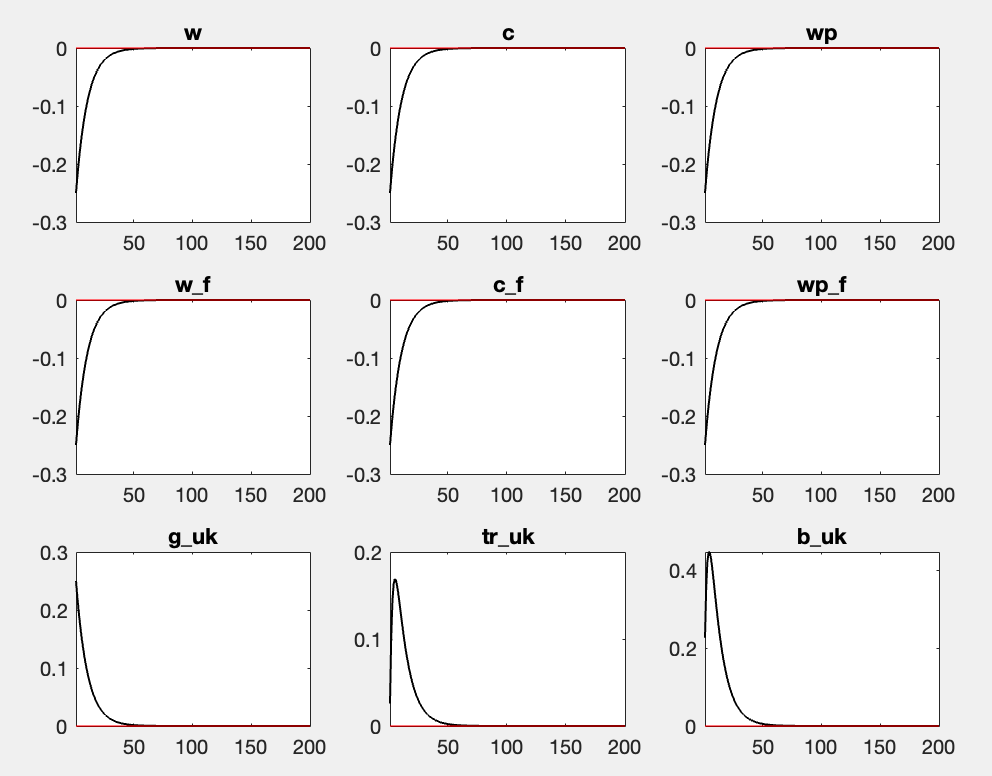
\includegraphics[width=\textwidth]{SCR-20230720-nhbg}